\documentclass[twoside,a4paper]{article}
\usepackage[utf8]{inputenc}
%\usepackage[uebung, answers]{tumbgdm}
\usepackage[klausur]{tumbgdm}
\Professor{Prof. Dr. Martin Werner}
\Universitaet{Technical University of Munich}
\Institut{School of Engineering and Design}
\Lehrstuhl{Professorship Big Geospatial Data Management}
\Semester[SuTe 2022]{Summer Term 2022}
\Vorlesung{Computational Foundations II}
\InstitutsWebsite{https://www.bgd.lrg.tum.de/}
\VorlesungsWebsite{https://www.moodle.tum.de/course/view.php?id=72588}
\usepackage{pdfpages}
%\nummerUebungsblatt{6}
%\nummerErsteFrage{14}
\klausurTitle{Exam Computational Foundations II \\(LRG0061, Summer Term 2022)}
%\LearningOutcome{
%We are warming up with C/C++ programming environments.
%}
\lstset{numbers=left, stepnumber=1}
\begin{document}

\maketitle
% 90 points for 90 minutes
\evaluationtable

\clearpage

\begin{task}{Multiple Choice}{5}{}
  Answer the following questions with yes or no. \\
  \emph{A wrong answer is counted as -1, a correct answer is counted as +1, an answer not given is counted as 0 (if you don't know the answer it is smarter not to give an answer!). If you reach more than 5 points, the points will become bonus points, if you reach less than 0 points, the result is 0 points.}
  \vspace{2cm}
  
\begin{mclist}
%  \mcquestion{In MATLAB, subsets of data can be created with slicing.}{X}{}{}
% \mcquestion{In MATLAB, one needs to allocate memory for an object before creating or using it using malloc and free.}{}{X}{}
% \mcquestion{For arbitrary large $n$, an algorithm of runtime complexity $O(n)$ will become faster than an algorithm of $O(n^2)$.}{X}{}{Of course}
% \mcquestion{The SDL libraries are a collection of linear algebra routines such that we can easily solve numeric problems in C++.}{}{X}{SDL = Simple Direct Media Layer = simple GUI framework.}
% \mcquestion{MATLAB is a compiled language generating native executables.}{}{X}{}
% \mcquestion{C++ is a compiled language generating native executables.}{X}{}{}
  % \mcquestion{A complete binary tree with depth $n$ has $2^n$ leaf nodes.}{X}{}{}
  \mcquestion{IEEE standard for floating point numbers (754) supports certain special values like infinity.}{X}{}{}
  \mcquestion{A 4-bit signed integer ranges from including -7 to including 8.}{}{X}{}
  \mcquestion{When adding two 8-bit numbers, the result can be held in 9 bit.}{X}{}{}
  \mcquestion{For computing the shortest path between all nodes of a graph, one typically runs Dijkstra with each node as the starting point}{}{X}{}
  \mcquestion{Binary Search is performing a search on ordered datasets by looking at the (approximately) middle data and continuing in each iteration with only (roughly) half of the array size. }{X}{}{}
  \mcquestion{The SPI bus is a communication system for connecting devices using 4 lanes ($SCLK,\overline{CS}, MISO, MOSI$)}{X}{}{}
  \mcquestion{In merge sort, the data is first cut into pieces for being sorted and the sorted pieces are assembled to a sorted version of the data.}{X}{}{}
  \end{mclist}
\end{task}
\clearpage
\begin{task}{Quadrature Phase Shift Keying}{5}{}
  The idea of the QPSK phase shift keying is that various phases represent different symbols, such that two bit are transmitted at the same time.

  \begin{enumerate}
  \item{Given a bitstring of 11011110, draw the modulation waveform in the following diagram and mark all keypoints (e.g., points where the waveform intersects the organizational lines) for better readability. Each symbol of two bit shall be transmitted with one roundtrip of the wave.

    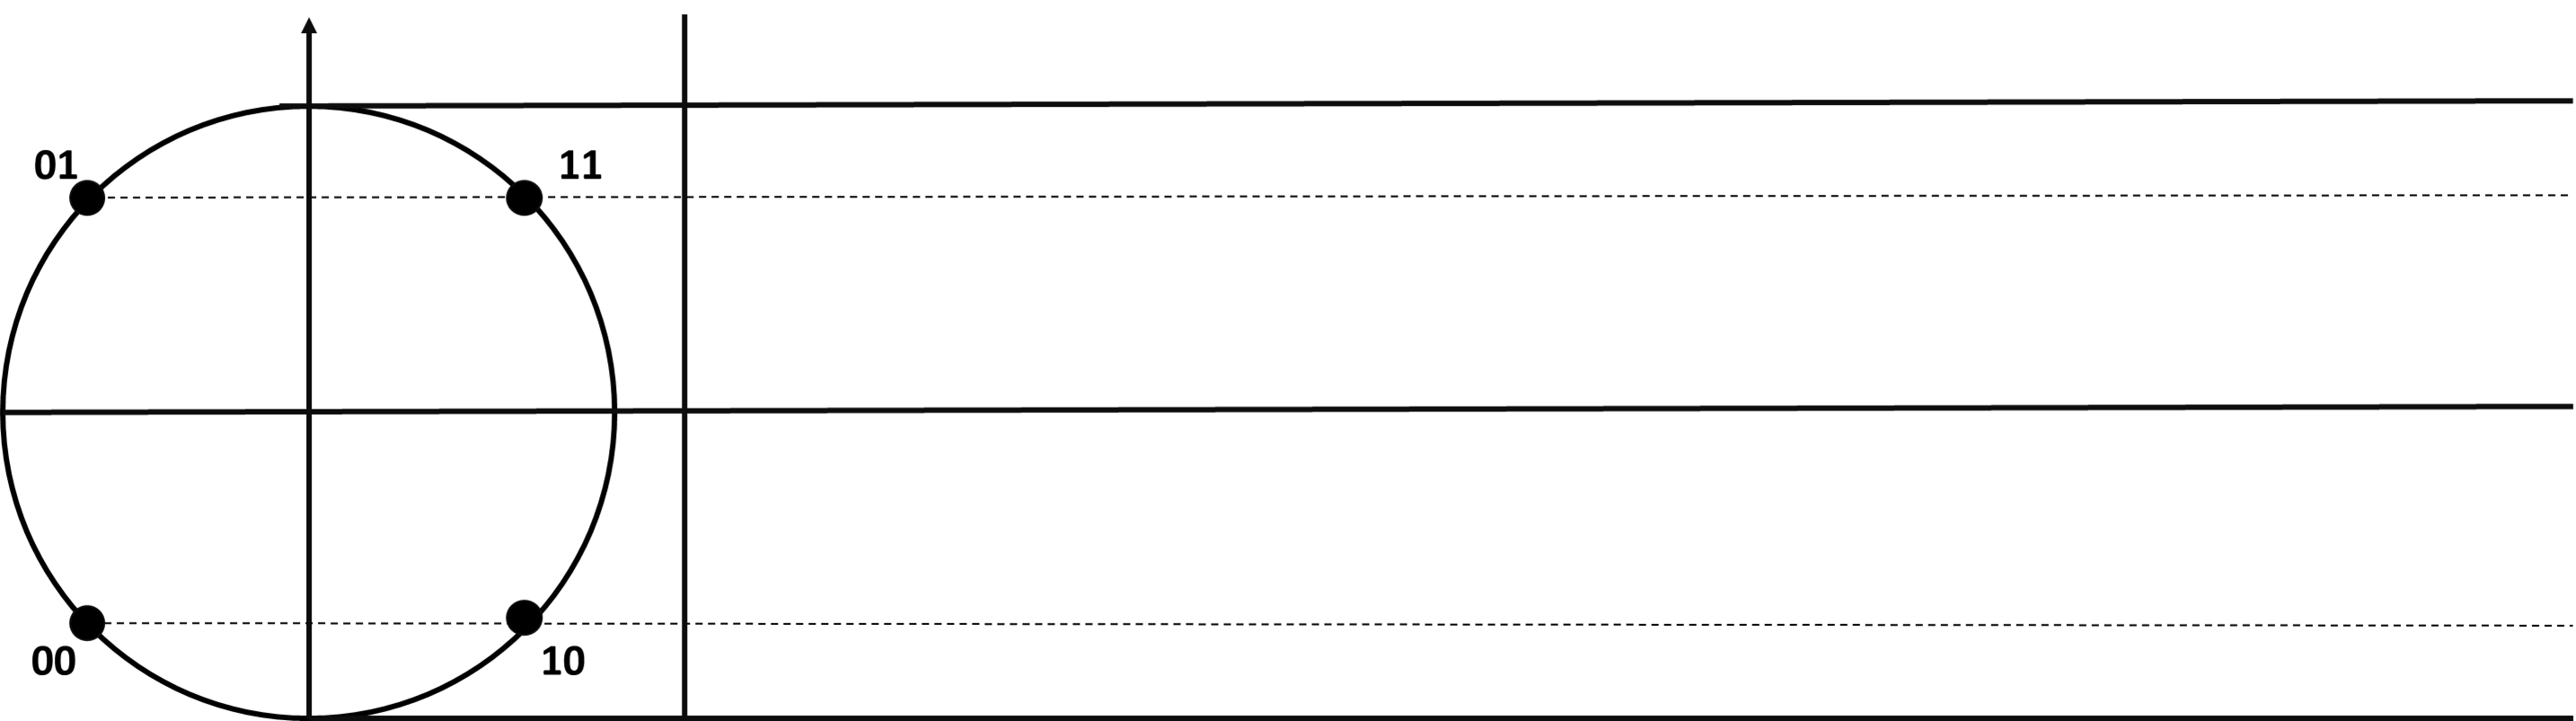
\includegraphics[width=\textwidth]{gfx/qpsk.png}

  }
  
    \end{enumerate}
\end{task}

\clearpage



\begin{task}{Number Representation}{10}{}

  Perform the following conversions into the number format:

  \begin{enumerate}
  \item{Represent 42 as an 8-bit unsigned integer (give all bits!)\vspace*{3cm}}
  \item{Represent -42 as an 8-bit signed integer (give all bits!)\vspace*{3cm}}
  \item{Represent 1.2 in IEEE Floating Point using 1 bit for the sign, 8 bit for the exponent, and 23 bits for the
    mantissa.\vspace*{3cm}}
\end{enumerate}
\end{task}


\clearpage
\begin{task}{Analog Digital Conversion}{10}{}
  % Convert some signal to int2.
  Analog Digital Conversion converts analogous signals into a digital representation. Explain the following two aspects
  each in one sentence:

  \begin{enumerate}
  \item{Quantization:\vspace*{6cm}}

    \item{Sampling: \vspace*{6cm}}

    \end{enumerate}
  
  
\end{task}
\clearpage
\begin{task}{Circuit Analysis}{10}{}
  Consider the following two circuits. 

  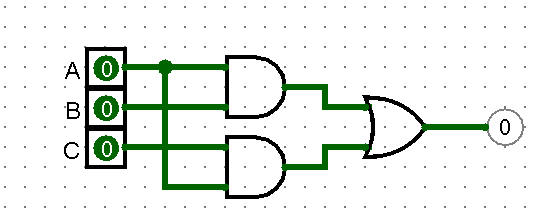
\includegraphics[width=.5\textwidth]{gfx/distributiv_circuit1.png}\\ \textbf{Circuit 1 (C1)}\par
  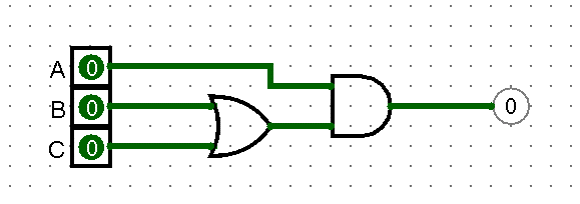
\includegraphics[width=.5\textwidth]{gfx/distributiv_circuit2.png}\\ \textbf{Circuit 2 (C2)}\par

  \begin{enumerate}
  \item{Show that they implement the same Boolean function using truth tables. \vspace*{6cm}}
  \item{Show that they implement the same Boolean function using algebraic identities \vspace*{2cm}}
    
  \end{enumerate}
  

  
\end{task}
\clearpage
\begin{task}{4-to-1 Multiplexer}{10}{}

  The 4-to-1 multiplexer is a simple combinatorial circuit which can be described as follows:
  Given four data input bits $(A_0,A_1,A_2,A_3)$ and two inputs $(S_1,S_2)$, the circuit interprets the inputs
  as an unsigned integer value in Big Endian bit order (as in the usual number system, the first digit $S_1$
  represents a higher value as opposed to the second digit $S_2$). A single output is filled with the current value
  of the input $A_i$ with $i$ being said value interpreted from $S_i$.

  \begin{enumerate}
  \item{
    Give the circuit as a truth table. In this table, treat $S_i$ as inputs and use the symbols $A_i$ for outputs that depend on $A_i$.
    \vspace*{6cm}}
  \item{Implement this circuit. Feel free to use multi-input versions of AND and OR.\clearpage }
    

    \end{enumerate}
\end{task}
\clearpage

\begin{task}{State Machines}{3}{}
  A state machine is a programming model in which two combinatorial circuits are combined with a state memory in
  order to achieve very complex behaviour.

  \begin{enumerate}
  \item{Give names or very short descriptions for the two combinatorial circuits\vspace{6cm}}
  \end{enumerate}
\end{task}

\clearpage
% TYPOS inside, otherwise a good task
%\begin{task}{Binary Search}{10}{}
%  Binary Search is a basic algorithm with which the time of finding an element in a vector can be reduced from an expecation of $\frac{N}{2} = O(N)$ to $\log O(N)$ making this approach much faster for large arrays.
%
%  Assume you are given an array $A$ with $N$ entries sorted by value.
%
%  \begin{enumerate}
%  \item{Describe, how binary search proceeds to find a value $v$ (you can assume it is in the array).\vspace*{6cm}}
%  \item{Assuming a sorting algorithm of $O(n \log n)$, given an \emph{unsorted} array, which approach is expected to be faster: (a) first sort the array, then use binary search or (b) directly search by looking at all elements ($O(n)$) \footnote{Note that Quantum Computers change this landscape as they allow a sublinear algorithm for non-sorted data. In fact, a suitably large QC can use Grover's algorithm to find an element in $O(\sqrt{N})$ time.}}
%  \end{enumerate}
%  
%\end{task}
%\clearpage
\begin{task}{Dijkstra}{10}{}
  Consider the diagram below.

  \centering{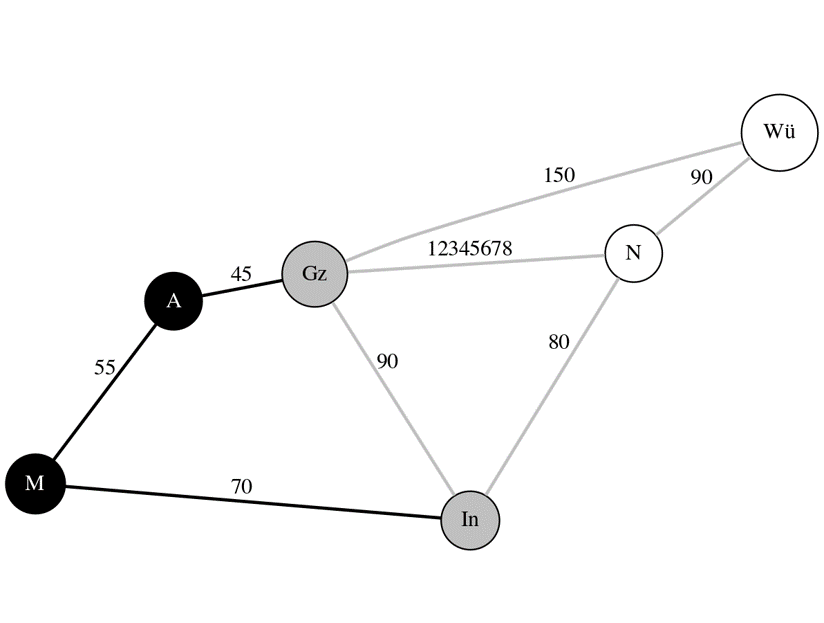
\includegraphics[width=.5\textwidth]{gfx/dijkstra.png}}

  Given our formulation of Dijkstra, answer the following questions:
  \begin{enumerate}
  \item{Give the Queue contents. Remember, that elements in the queue are pairs of a vertex and a weight and that the queue is sorted.
\vspace*{2cm}
  }
  \item{Give the complete distance map and the complete predecessor map at the moment in the diagram. Remember, that the distance map is initialized to $\infty$ and that the predecessor map is initialized such that for every vertex we store the vertex itself.

    \parbox{.5\textwidth}{\textbf{Distance Map (d)}\par
      \vspace*{1em}\Large\begin{tabular}{|c|c|}
        \hline
        \textbf{Node} & \textbf{Value} \\ \hline
        M & 0 \\ \hline
        A & \\ \hline
        In & \\ \hline
        Gz & \\ \hline
        N & \\ \hline
        Wü & \\ \hline
        \end{tabular}
        }
    \parbox{.5\textwidth}{\textbf{Predecessor Map (p)}\par
      \vspace*{1em}\Large\begin{tabular}{|c|c|}
        \hline
        \textbf{Node} & \textbf{Value} \\ \hline
        M & M \\ \hline
        A & \\ \hline
        In & \\ \hline
        Gz & \\ \hline
        N & \\ \hline
        Wü & \\ \hline
        \end{tabular}
        }


    \vspace{1cm}}
    \item{The $A^*$ algorithm is considered to be faster than Dijkstra in many scenarios. What is the additional information it exploits?\vspace{3cm}}
    \end{enumerate}
  

  \end{task}

\end{document}
